In the study context, the Raw Task Load Index (Raw-TLX) is used as a simplified
version of the NASA Task Load Index (NASA-TLX). One potential difference is
that NASA-TLX incorporates a weighting process to adjust each scale to an
individual's perception of workload \cite{hart1988development}. In contrast,
Raw-TLX omits this weighting process to maintain simplicity and ease of
application \cite{hart2006nasa}.

In alignment with the use of Raw-TLX, the study also omitted one of the scales,
Physical Demand, as it did not apply to the specific context of the task. The
omission of this scale was due to its lack of relevance in assessing the
workload associated with the decomposition tasks in the study. Not omitting the
scale could skew the overall score since all scales have equal weight, that is,
\( \frac{100}{6} \).

The Raw Task Load Index (Raw-TLX) was conducted to collect information on the
effort required to complete the monolith decomposition tasks using the
application. Then we calculated each category's average and median scores
separately for each task. Task 1 and 2 results and scores are presented in
\Cref{tab:separated_task_1,tab:separated_task_2} as well as visualy in
\Cref{fig:separated_task_1,fig:separated_task_2}, respectively.

\Cref{tab:tasks_results} combines Task 1 and Task 2 results and the general
average and median to provide a comprehensive overview of the perceived
workload across both tasks. The visualisation in \Cref{fig:tasks_results}
allows for comparing and analysing the workload distribution across the
different categories for the overall study.

\begin{table}[!htb] \caption{Task 1 Results Table} \label{tab:separated_task_1}
  \begin{center}
    \begin{tabular}[c]{p{4em}|p{4em}|p{4em}|p{4em}|p{4em}|p{4em}}
      \textbf{} &
      \textbf{Mental Demand} &
      \textbf{Temporal Demand} &
      \textbf{Perfor\-mance} &
      \textbf{Effort} &
      \textbf{Frustration} \\
      \hline Average & 4.71 & 4.14 & 4.71 & 4.86 & 3.43 \\
      \hline Median & 5.0 & 4.0 & 4.0 & 5.0 & 3.0 \\
    \end{tabular}
  \end{center}
\end{table}

\begin{figure*}[!htb]
  \caption{Task 1 Graph}
  \label{fig:separated_task_1}
  \centering
  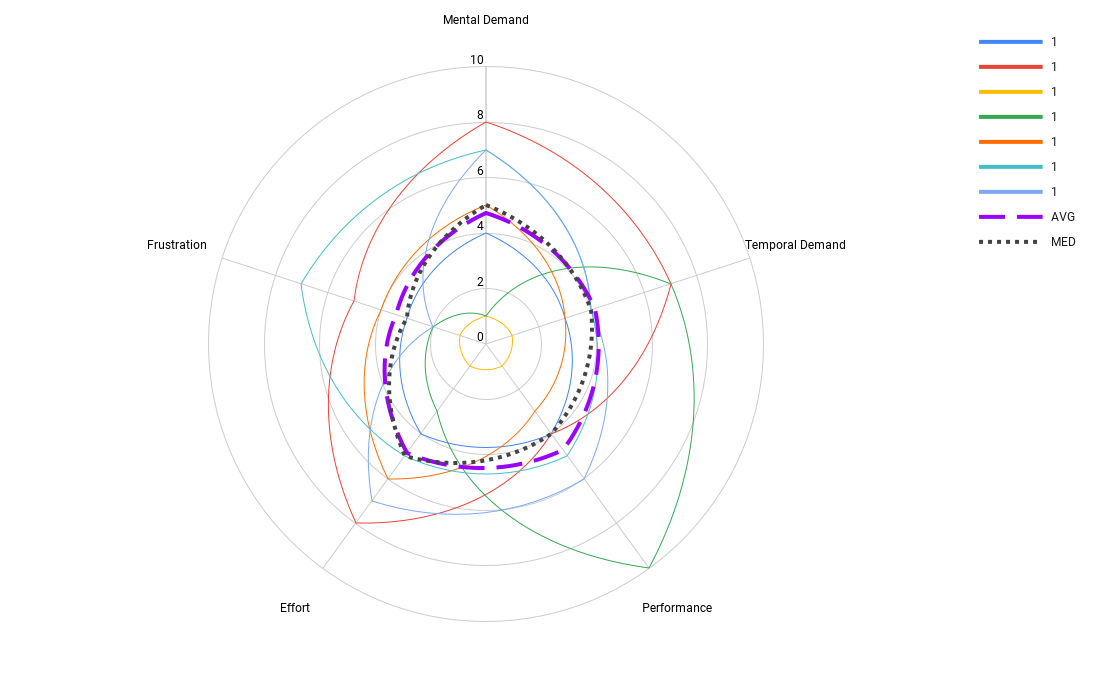
\includegraphics[width=\textwidth]{task1_results}
\end{figure*}

\begin{table}[!htb] \caption{Task 2 Results Table} \label{tab:separated_task_2}
  \begin{center}
    \begin{tabular}[c]{p{4em}|p{4em}|p{4em}|p{4em}|p{4em}|p{4em}}
      \textbf{} &
      \textbf{Mental Demand} &
      \textbf{Temporal Demand} &
      \textbf{Performance} &
      \textbf{Effort} &
      \textbf{Frustration} \\
      \hline Average & 4.13 & 4.75 & 5.75 & 5.00 & 3.25 \\
      \hline Median & 4.0 & 5.0 & 7.0 & 5.5 & 2.5 \\
    \end{tabular}
  \end{center}
\end{table}

\begin{figure*}[!htb]
  \caption{Task 2}
  \label{fig:separated_task_2}
  \centering
  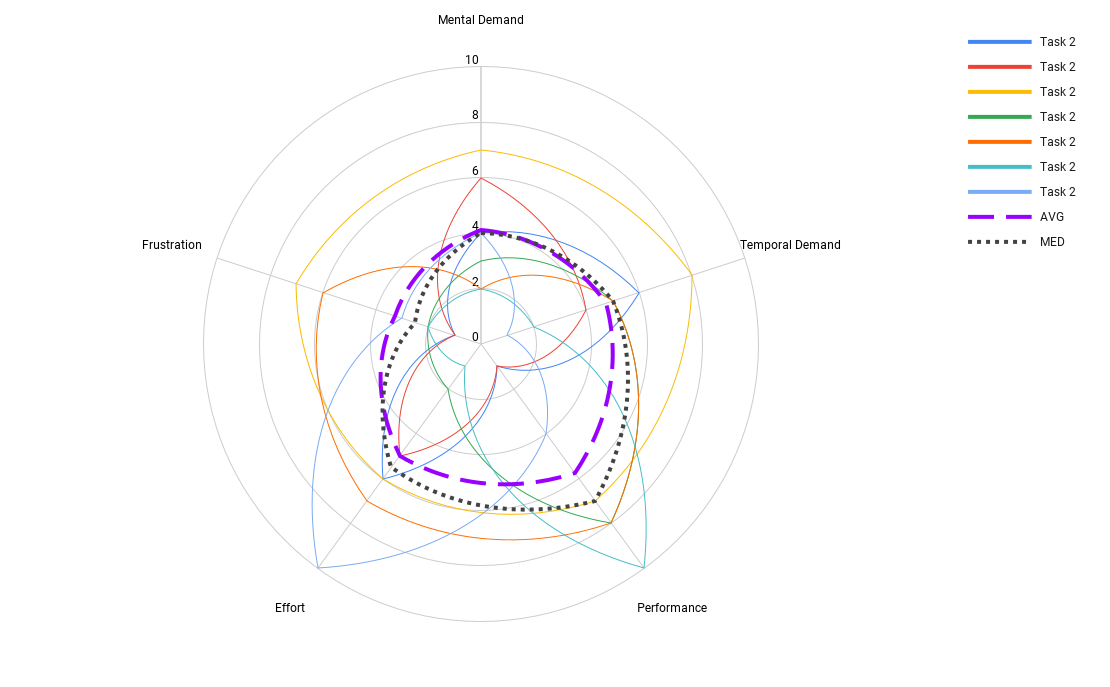
\includegraphics[width=\textwidth]{task2_results}
\end{figure*}

\begin{table}[!htb] \caption{Tasks Results Table} \label{tab:tasks_results}
  \begin{center}
    \begin{tabular}[c]{p{4em}|p{4em}|p{4em}|p{4em}|p{4em}|p{4em}}
      \textbf{} &
      \textbf{Mental Demand} &
      \textbf{Temporal Demand} &
      \textbf{Perfor\-mance} &
      \textbf{Effort} &
      \textbf{Frustration} \\
      \hline Average & 4.40 & 4.47 & 5.27 & 4.93 & 3.33 \\
      \hline Median & 4.0 & 4.0 & 5.0 & 5.0 & 3.0 \\
    \end{tabular}
  \end{center}
\end{table}

\begin{figure*}[!htb]
  \caption{Tasks Results}
  \label{fig:tasks_results}
  \centering
  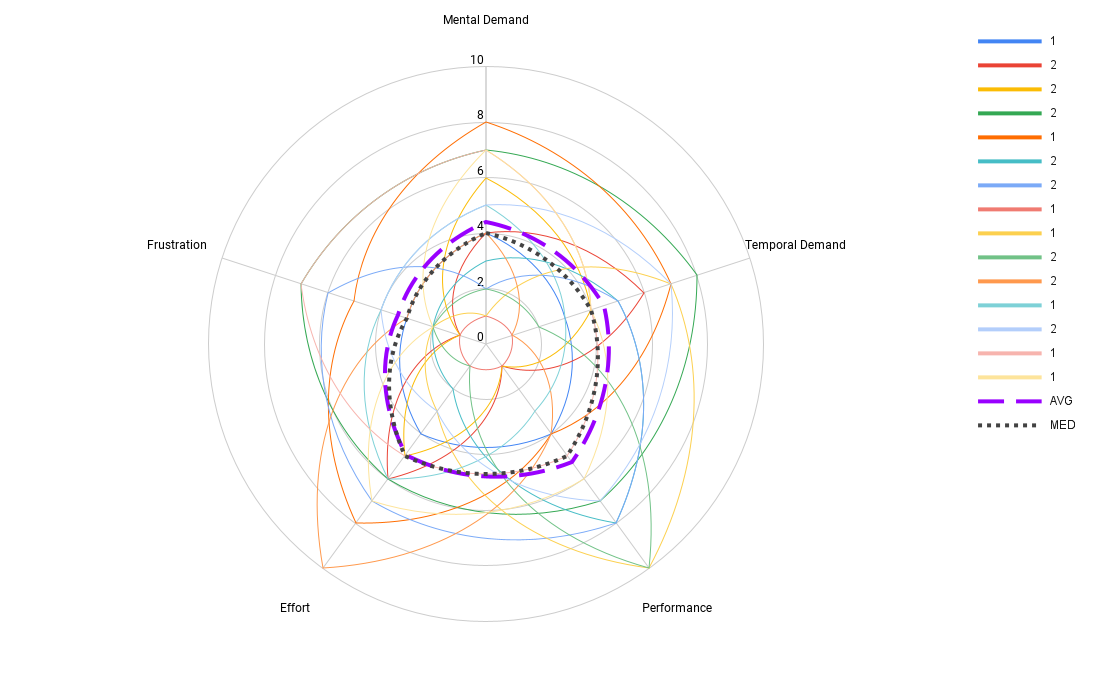
\includegraphics[width=\textwidth]{tasks_results}
\end{figure*}
